\colorfulheader{computer vision}

\begin{minipage}{0.485\textwidth}
\textbf{Convolution} is a mathematical operation on two function $\parenthesisA{f\text{and }g}$ that produces a third function $\parenthesisA{f*g}$ that expresses \textit{how the shape of one is modified by the other}. Formally,
\begin{align*}
    \parenthesisA{f*g}\parenthesisA{t} = \int_{-\infty}^{+\infty}f\parenthesisA{\tau}g\parenthesisA{t - \tau}d\tau
\end{align*}
\end{minipage}
\hspace{10pt}
\begin{minipage}{0.485\textwidth}
It can be generalized to $n$ dimensions and in practice the integral can be changed for a summation $\parenthesisA{\sum}$ and the integral limits defined by the problem's context to do a \textbf{discrete convolution}. For example, a 2D convolution in image processing would be
\begin{align*}
    \text{Conv2D}\parenthesisA{x,y} = \sum_{i=-\frac{n}{2}}^{\frac{n}{2}}\sum_{j=-\frac{m}{2}}^{\frac{m}{2}}h\parenthesisA{i,j}I\parenthesisA{x - i, y - j}
\end{align*}
\end{minipage}
\begin{minipage}{\textwidth}
\vspace{5pt}
\begin{center}
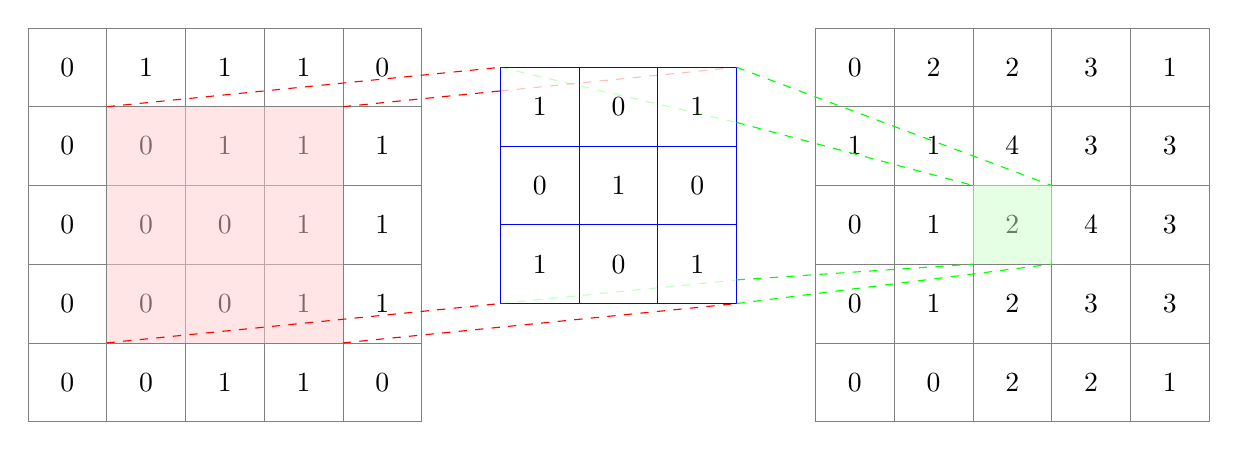
\begin{tikzpicture}
\draw[step=1cm,gray,very thin] (0,0) grid (5,5);
\node[] at (0.5,0.5){0};
\node[] at (1.5,0.5){0};
\node[] at (2.5,0.5){1};
\node[] at (3.5,0.5){1};
\node[] at (4.5,0.5){0};
\node[] at (0.5,1.5){0};
\node[] at (1.5,1.5){0};
\node[] at (2.5,1.5){0};
\node[] at (3.5,1.5){1};
\node[] at (4.5,1.5){1};
\node[] at (0.5,2.5){0};
\node[] at (1.5,2.5){0};
\node[] at (2.5,2.5){0};
\node[] at (3.5,2.5){1};
\node[] at (4.5,2.5){1};
\node[] at (0.5,3.5){0};
\node[] at (1.5,3.5){0};
\node[] at (2.5,3.5){1};
\node[] at (3.5,3.5){1};
\node[] at (4.5,3.5){1};
\node[] at (0.5,4.5){0};
\node[] at (1.5,4.5){1};
\node[] at (2.5,4.5){1};
\node[] at (3.5,4.5){1};
\node[] at (4.5,4.5){0};
\fill[red!20!white,semitransparent] (1,1) rectangle (4,4);
\draw[red,dashed] (1,1) -- (6,1.5);
\draw[red,dashed] (4,1) -- (9,1.5);
\draw[red,dashed] (1,4) -- (6,4.5);
\draw[red,dashed] (4,4) -- (6,4.2);
\draw[red,dashed,nearly transparent] (6,4.2) -- (9,4.5);
% \foreach \x in {0,...,4}{
%     \foreach \y in {0,...,4}{
%         \pgfmathsetmacro\result{\x+(\y*4)}
%         \node[gray] at (0.5+\x,0.5+\y){\pgfmathprintnumber{\result}};
%     }
% }
\draw[blue,xshift=5cm,yshift=0.5cm] (1,1) grid (4,4);
\node[xshift=5cm,yshift=0.5cm] at (1.5,1.5){1};
\node[xshift=5cm,yshift=0.5cm] at (2.5,1.5){0};
\node[xshift=5cm,yshift=0.5cm] at (3.5,1.5){1};
\node[xshift=5cm,yshift=0.5cm] at (1.5,2.5){0};
\node[xshift=5cm,yshift=0.5cm] at (2.5,2.5){1};
\node[xshift=5cm,yshift=0.5cm] at (3.5,2.5){0};
\node[xshift=5cm,yshift=0.5cm] at (1.5,3.5){1};
\node[xshift=5cm,yshift=0.5cm] at (2.5,3.5){0};
\node[xshift=5cm,yshift=0.5cm] at (3.5,3.5){1};
\draw[step=1cm,gray,very thin,xshift=10cm] (0,0) grid (5,5);
\node[xshift=10cm] at (0.5,0.5){0};
\node[xshift=10cm] at (1.5,0.5){0};
\node[xshift=10cm] at (2.5,0.5){2};
\node[xshift=10cm] at (3.5,0.5){2};
\node[xshift=10cm] at (4.5,0.5){1};
\node[xshift=10cm] at (0.5,1.5){0};
\node[xshift=10cm] at (1.5,1.5){1};
\node[xshift=10cm] at (2.5,1.5){2};
\node[xshift=10cm] at (3.5,1.5){3};
\node[xshift=10cm] at (4.5,1.5){3};
\node[xshift=10cm] at (0.5,2.5){0};
\node[xshift=10cm] at (1.5,2.5){1};
\node[xshift=10cm] at (2.5,2.5){2};
\fill[green!20!white,semitransparent,xshift=10cm] (2,2) rectangle (3,3);
\node[xshift=10cm] at (3.5,2.5){4};
\node[xshift=10cm] at (4.5,2.5){3};
\node[xshift=10cm] at (0.5,3.5){1};
\node[xshift=10cm] at (1.5,3.5){1};
\node[xshift=10cm] at (2.5,3.5){4};
\node[xshift=10cm] at (3.5,3.5){3};
\node[xshift=10cm] at (4.5,3.5){3};
\node[xshift=10cm] at (0.5,4.5){0};
\node[xshift=10cm] at (1.5,4.5){2};
\node[xshift=10cm] at (2.5,4.5){2};
\node[xshift=10cm] at (3.5,4.5){3};
\node[xshift=10cm] at (4.5,4.5){1};
\draw[green,dashed] (9,1.5) -- (13,2);
\draw[green,dashed] (9,4.5) -- (13,3);
\draw[green,dashed,nearly transparent] (6,1.5) -- (9,1.8);
\draw[green,dashed] (9,1.8) -- (12,2);
\draw[green,dashed,nearly transparent] (6,4.5) -- (9,3.8);
\draw[green,dashed] (9,3.8) -- (12,3);
\end{tikzpicture}
\end{center}
\end{minipage}
\begin{figure}[h]
\begin{center}
\begin{minipage}{0.5\textwidth}
    \begin{lstlisting}[frame=single]
    bool outOfBounds(int n, int m, int w, int h)
    {
      return (n < 0 || n > h - 1 || m < 0 || m > w - 1);
    }
    typedef vector<vector<int>> vvint;
    vvint convolution2D(const vvint & M, const vvint & K)
    {
      vvint convolution;
      int height = M.size();
      int width = M[0].size();
      int n2 = K.size() / 2;
      int m2 = K[0].size() / 2;
      convolution.resize(M.size());
      for (int n = 0; n < height; n++)
      {
        convolution[n].resize(width);
        for (int m = 0; m < width; m++)
        {
          int sum = 0;
          for (int i = -n2; i <= n2; i++) 
          {
            for (int j = -m2; j <= m2; j++) 
            {
              // Clamp result in bounds
              if (!outOfBounds(n - i, m - j, width, height))
              {
                sum += (K[i + n2][j + m2] * M[n - i][m - j]);
              }
            }
          }
        convolution[n][m] = sum;
        }
      }
      return convolution;
    }
    \end{lstlisting}
\end{minipage}
\hspace{10pt}
\begin{minipage}{0.465\textwidth}
    \textbf{Computer Vision} is the area of inferring properties given an image. Its pipeline can be simplified as
    \begin{center}
        \resizebox{9cm}{9cm}{
        \begin{tikzpicture}
            \node (cv1) [text centered,text width=7cm,fill=purple!20] {\textbf{Specify Image} \\ \vspace{-6pt}\rule{\textwidth}{1pt} \\ $[\underbrace{\texttt{RGB,CYK}}_{\text{Color Model}}\dots\underbrace{\texttt{PNG,JPG}}_{\text{Compression}}\dots\underbrace{\texttt{uint32,float}}_{\text{Data Type}}\dots]$};
            \node (cv2) [text centered,text width=9.5cm,fill=blue!20,below of=cv1,yshift=-1.1cm] {\textbf{Pre-processing} \\ \vspace{-6pt}\rule{\textwidth}{1pt} \\ $[\underbrace{\text{Resize \textbar\hspace{3pt}Reshape}}_{\text{Aspect Ratio, ROI, etc.}}, \underbrace{\text{Transformations}}_{\text{Rotation, Reflection, etc.}}, \underbrace{\text{RGB To Gray}}_{\text{Mapping, Filtering, etc.}}]$};
            \node (cv3) [text centered, text width=7cm,fill=green!20,below of=cv2,yshift=-2.5cm] {\textbf{Algorithm} \\ \vspace{-6pt}\rule{\textwidth}{1pt} \\ $\underbrace{\text{Transformations}}_{\substack{\text{Convolution} \\ \text{Discrete Fourier Transform} \\ \text{Histograms}}}$ \\ Segmentation \\ Optical Flow \textbar\hspace{2pt} Tracking \\ Camera Calibration \textbar\hspace{2pt} Undistorsion \\ $\underbrace{\text{SFM}}_{\substack{\text{Structure} \\ \text{From Motion}}}$ \textbar\hspace{2pt} $\underbrace{\text{SLAM}}_{\substack{\text{Simultaneous} \\ \text{Location And} \\ \text{Mapping}}}$};
            \node (cv4) [text centered,text width=10cm,fill=yellow!20,below of=cv3,yshift=-2.45cm] {\textbf{Post-processing} \\ \vspace{-6pt}\rule{\textwidth}{1pt} \\ $[\text{Some as pre-processing}, \underbrace{\text{Kernels \textbar\hspace{3pt}Matrix Operators}}_{\text{Blurring, Smoothing Sharpening, etc.}}]$};
            \node (cv5) [text centered,fill=red!20,below of=cv4,yshift=-0.5cm] {\textbf{Display}};
            \draw [arrow] (cv1) -- node[anchor=south]{} (cv2);
            \draw [arrow] (cv2) -- node[anchor=south]{} (cv3);
            \draw [arrow] (cv3) -- node[anchor=south]{} (cv4);
            \draw [arrow] (cv4) -- node[anchor=south]{} (cv5);
        \end{tikzpicture}
        }
    \end{center}
    Relevant \textbf{kernels}
    \begin{align*}
        &
        \overbrace{
        \underbrace{
        \frac{1}{9}
        \begin{bmatrix}
        1 & 1 & 1 \\
        1 & 1 & 1 \\
        1 & 1 & 1
        \end{bmatrix}
        }_{\text{Box}}
        \underbrace{
        \frac{1}{16}
        \begin{bmatrix}
        1 & 2 & 1 \\
        2 & 4 & 2 \\
        1 & 2 & 1
        \end{bmatrix}
        }_{\text{Gaussian}}
        }^{\text{Blur}}
        \overbrace{
        \underbrace{
        \begin{bmatrix}
        0 &  1 & 0 \\
        1 & -4 & 1 \\
        0 &  1 & 0 \\
        \end{bmatrix}
        }_{\text{Laplacian}}
        }^{\text{Sharpening}} \\
        &
        \overbrace{
        \underbrace{
        \overbrace{
        \begin{bmatrix}
        i^2 & 0 & 1 \\
        i^2 & 0 & 1 \\
        i^2 & 0 & 1
        \end{bmatrix}
        }^{x}
        \overbrace{
        \begin{bmatrix}
        i^2 & i^2 & i^2 \\
         0 &  0 &  0 \\
         1 &  1 &  1
        \end{bmatrix}
        }^{y}
        }_{\text{Prewitt}}
        \underbrace{
        \overbrace{
        \begin{bmatrix}
        -1 & 0 & 1 \\
        -2 & 0 & 2 \\
        -1 & 0 & 1
        \end{bmatrix}
        }^{x}
        \overbrace{
        \begin{bmatrix}
        -1 & -2 & -1 \\
        0 & 0 & 0 \\
        1 & 2 & 1
        \end{bmatrix}
        }^{y}
        }_{\text{Sobel}}
        }^{\text{Edge Detection}}
    \end{align*}
\end{minipage}
\end{center}
\end{figure}